\documentclass[../../../main.tex]{subfiles}
\begin{document}

Throughout this manuscript, the complete development of the algorithm for generating self-sustaining stochastic porous structures has been explained. 
The initial ideas developed to achieve the sought objective have been presented, along with evidence that these solutions were not valid. 
Subsequently, the final state reached by distilling these initial ideas is described in detail. 
All the components that form part of this algorithm are explained in the Methodology section of this manuscript. 
However, at no point is the potential of this algorithm for generating stochastic structures revealed, nor are its limitations disclosed. 
This section aims to provide an overview of all the modules that make up the package developed throughout this project. 
In addition, a study is included on how the behaviour of the structures obtained varies for different values of the design parameters.

\subsection{Mesh-gen: Python package modules and their integration}

All the algorithms developed during this work have been included in a Python package called \textit{mesh-gen}. 
Any reader interested in its use and operation can access it to complete all the concepts explained in the methodology of this work. 
In addition, the algorithms used to perform the matrix calculation of reticular structures and their optimisation have been published in another module, Spyffness. 
The main package consists of two main modules and a third module for generating the G-code that allows the generated structure to be printed in a non-planar form. 
This third module has not been integrated into the overall flow, in case the user is not interested in printing the structure this way. 
The names of the files will not be mentioned, as the package developed will continue to be maintained and evolved after the completion of this doctoral thesis, and some names may change. 

Before the modules are executed, a script is executed to check that all the necessary configuration for the correct execution of the package is defined. 
The logger is initialised and the execution folders are created, where all the files generated during execution will be saved: logs, graph and STL file.
Next, it checks whether there is a graph stored in the temporary folder. 
If so, the first module is not executed, and the graph stored in the temporary folder is used to generate the STL file. 
This was implemented to avoid duplicate executions and thus speed up overall execution. 
If there is no graph stored in the temporary folder, the geometry entered is processed, the points and sections of interest are extracted, and the first module is executed

The first module is responsible for generating the skeleton of the structure. 
This module receives as input the points and sections of the geometry to be processed and the values defined as the minimum allowed angle and pore size.
Next, all the routines that carry out the procedures explained in the methodology are executed. 
After obtaining the skeleton of the structure, it is saved in a pickle file as a Networkx object both in the folder created for execution and in the temporary folder, and the second module is executed.

The second module is responsible for generating the mesh of the generated structure. 
Within the configuration file, the user can choose whether or not to generate a fused mesh. 
If so, this module executes George W. Hart's modified algorithm and generates a mesh that is saved as an STL file. 
If not, a mesh will be generated based on the positioning of cylinders on the edges, which will not be joined, but is valid for printing the structure in 3D.
\cref{fig:workflow} shows a diagram of the overall flow of the main modules. To avoid redundancy of images, a flow for the case in which a merged mesh is not generated is not included, as the other case shown is more complete. This case would only include a step for generating the cylinders and another for exporting the STL file. The thickness of the cylinders or edges used in both cases is the same.

\begin{figure}[!htbp]
    \centering
    \\includegraphics[width= 0.8\textwidth]{imgs/workflow.svg.pdf}
    \caption{Overall workflow of the main modules of the mesh-gen package.}
    \label{fig:workflow}
\end{figure}

\subsection{Analysis of design parameters: minimum angle}

Although the objective of the developed algorithm is to generate self-supporting stochastic structures, the minimum angle that the edges can have was left as a design parameter so that it can be customised. 
While it is true that a 45$^\circ$ angle is sufficient to ensure self-sustainability, it is not necessarily the minimum angle that can be printed. 
Surfaces with smaller angles can also be printed under certain conditions. 
For example, if the printing speed is reduced and cooling is increased, it is possible to print with smaller angles. 
The minimum possible angle will always depend on the 3D printer and the printing conditions.
\cref{fig:angles} shows the angle distribution obtained for four different minimum angle values. 
It can be seen that there are effectively no edges with angles smaller than those established. 
In addition, the minimum angle is not the most common, but rather that it is usually approximately 5$^\circ$ greater than the minimum. 
There are very vertical angles that are usually present on the edges of the surface or on the last layer.  
This figure proves that the algorithm is capable of generating structures that ensure the self-sustainability of all edges.

\begin{figure}[!htbp]
    \centering
    \\includegraphics[width= 0.6\textwidth]{imgs/angles.svg.pdf}
    \caption{Distribution of angles obtained for four structures with different minimum allowed angle values.}
    \label{fig:angles}
\end{figure}

\subsection{Analysis of design parameters: pore area}

Another objective of the algorithm is to control the pore size in the generated structures. The definition of a pore is very ambiguous in reticular structures. 
It is difficult to define the physical limits that delimit the pore region. 
Closed-cell porous structures have a surface that partially or totally surrounds the pore, making it easy to define this region.
However, in reticular structures, there is no surface that can give an idea of the limits of this region. 
In regular reticular structures, the pore can be defined as the volume of the unit cell used to design the structure.
However, in the case of stochastic structures, there is no repeating unit cell from which to deduce porosity. 
In these cases, it is more common to define the structure by its relative porosity rather than its pore size.
However, relative porosity cannot be known a priori because, in this case, it depends on the size of the edges that will be used later. 
Therefore, it was decided to discard the use of the term \textit{pore size} or \textit{pore volume} and use \textit{pore area} instead. 

The pore area was defined as the average area of the polygons that make up any section of the structure. 
Therefore, assuming that the volume to be processed has a constant section, if the number of polygons in each layer is the same, the average area must also be the same. 
For this reason, in the first iteration of the algorithm, the lower section of the volume is extracted, and the necessary triangles are generated in it so that the average size of the areas is that indicated by the pore area parameter. 
This process sets the number of polygons that will have to be in the following layers. 
If the processed volume did not have a constant section, the number of polygons to be generated is recalculated based on the variation in area. 
This ensures that the ratio of the perimeter to the number of polygons is constant. 
To calculate the pore area, the area of each of the polygons that make up each of the sections is calculated. 
Each of the polyhedra generated is stored in a dictionary where their points are classified according to whether they are base or apex points. 
The base points are then triangulated, the area of the triangle face is calculated, and the sum of all the areas is obtained.
As the triangulations are performed using the projections of each of the points, the value of the areas obtained is the value of the area of the projection onto the horizontal plane of each of the triangles, see \cref{fig:aberration}. 
Therefore, to obtain the actual area, it is divided by the cosine of the minimum angle, as this will be the most common aberration value. 
So, to obtain the desired pore area value throughout the layers, the pore area parameter set must be multiplied by the cosine of the minimum angle. 

\begin{figure}[!htbp]
    \centering
    

\tikzset{every picture/.style={line width=0.75pt}} %set default line width to 0.75pt        

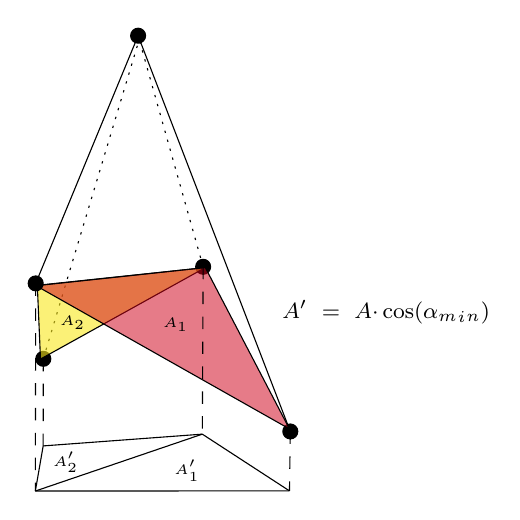
\begin{tikzpicture}[x=0.75pt,y=0.75pt,yscale=-1,xscale=1]
%uncomment if require: \path (0,300); %set diagram left start at 0, and has height of 300

%Shape: Circle [id:dp20203675621890882] 
\draw  [fill={rgb, 255:red, 0; green, 0; blue, 0 }  ,fill opacity=1 ] (75,183.4) .. controls (75,181.41) and (76.61,179.8) .. (78.6,179.8) .. controls (80.59,179.8) and (82.2,181.41) .. (82.2,183.4) .. controls (82.2,185.39) and (80.59,187) .. (78.6,187) .. controls (76.61,187) and (75,185.39) .. (75,183.4) -- cycle ;
%Shape: Circle [id:dp4460917567211786] 
\draw  [fill={rgb, 255:red, 0; green, 0; blue, 0 }  ,fill opacity=1 ] (152,139.07) .. controls (152,137.08) and (153.61,135.47) .. (155.6,135.47) .. controls (157.59,135.47) and (159.2,137.08) .. (159.2,139.07) .. controls (159.2,141.05) and (157.59,142.67) .. (155.6,142.67) .. controls (153.61,142.67) and (152,141.05) .. (152,139.07) -- cycle ;
%Shape: Circle [id:dp23372343609699975] 
\draw  [fill={rgb, 255:red, 0; green, 0; blue, 0 }  ,fill opacity=1 ] (194,218.4) .. controls (194,216.41) and (195.61,214.8) .. (197.6,214.8) .. controls (199.59,214.8) and (201.2,216.41) .. (201.2,218.4) .. controls (201.2,220.39) and (199.59,222) .. (197.6,222) .. controls (195.61,222) and (194,220.39) .. (194,218.4) -- cycle ;
%Shape: Circle [id:dp7435513334633294] 
\draw  [fill={rgb, 255:red, 0; green, 0; blue, 0 }  ,fill opacity=1 ] (120.67,27.73) .. controls (120.67,25.75) and (122.28,24.13) .. (124.27,24.13) .. controls (126.25,24.13) and (127.87,25.75) .. (127.87,27.73) .. controls (127.87,29.72) and (126.25,31.33) .. (124.27,31.33) .. controls (122.28,31.33) and (120.67,29.72) .. (120.67,27.73) -- cycle ;
%Straight Lines [id:da9245497792530712] 
\draw [color={rgb, 255:red, 0; green, 0; blue, 0 }  ,draw opacity=1 ] [dash pattern={on 0.84pt off 2.51pt}]  (78.6,183.4) -- (124.27,31.33) ;
%Straight Lines [id:da7005143254135355] 
\draw [color={rgb, 255:red, 0; green, 0; blue, 0 }  ,draw opacity=1 ] [dash pattern={on 0.84pt off 2.51pt}]  (155.6,139.07) -- (124.27,27.73) ;
%Straight Lines [id:da28064823401026573] 
\draw    (197.6,218.4) -- (124.27,27.73) ;
%Shape: Triangle [id:dp11918551614132744] 
\draw  [fill={rgb, 255:red, 248; green, 231; blue, 28 }  ,fill opacity=0.6 ] (77.24,183.52) -- (156.66,139.45) -- (75.71,148) -- cycle ;
%Shape: Triangle [id:dp7709931078112477] 
\draw  [fill={rgb, 255:red, 208; green, 2; blue, 27 }  ,fill opacity=0.52 ] (197.19,217.19) -- (75.12,148.19) -- (156.66,139.45) -- cycle ;
%Straight Lines [id:da7697818424224974] 
\draw [fill={rgb, 255:red, 0; green, 0; blue, 0 }  ,fill opacity=1 ]   (74.93,147.07) -- (124.27,27.73) ;
%Shape: Circle [id:dp25664476075983755] 
\draw  [fill={rgb, 255:red, 0; green, 0; blue, 0 }  ,fill opacity=1 ] (71.33,147.07) .. controls (71.33,145.08) and (72.95,143.47) .. (74.93,143.47) .. controls (76.92,143.47) and (78.53,145.08) .. (78.53,147.07) .. controls (78.53,149.05) and (76.92,150.67) .. (74.93,150.67) .. controls (72.95,150.67) and (71.33,149.05) .. (71.33,147.07) -- cycle ;
%Straight Lines [id:da5723635368812333] 
\draw  [dash pattern={on 4.5pt off 4.5pt}]  (74.93,147.07) -- (74.76,247.11) ;
%Straight Lines [id:da9477555281674963] 
\draw  [dash pattern={on 4.5pt off 4.5pt}]  (78.6,183.4) -- (78.53,225.37) ;
%Straight Lines [id:da7265146935260219] 
\draw  [dash pattern={on 4.5pt off 4.5pt}]  (155.6,139.07) -- (155.2,219.7) ;
%Straight Lines [id:da8482223625070795] 
\draw  [dash pattern={on 4.5pt off 4.5pt}]  (197.6,218.4) -- (197.2,247.03) ;
%Straight Lines [id:da135198346268814] 
\draw    (74.76,247.11) -- (197.2,247.03) ;
%Straight Lines [id:da7899881746363868] 
\draw    (155.2,219.7) -- (197.2,247.03) ;
%Straight Lines [id:da24200805108322687] 
\draw    (74.76,247.11) -- (155.2,219.7) ;
%Straight Lines [id:da38438776639593253] 
\draw    (78.53,225.37) -- (74.76,247.11) ;
%Straight Lines [id:da27704931617334616] 
\draw    (155.2,219.7) -- (78.53,225.37) ;

% Text Node
\draw (135,162.5) node [anchor=north west][inner sep=0.75pt]  [font=\tiny] [align=left] {$\displaystyle A_{1}$};
% Text Node
\draw (140.5,231) node [anchor=north west][inner sep=0.75pt]  [font=\tiny] [align=left] {$\displaystyle A'_{1}$};
% Text Node
\draw (82,227) node [anchor=north west][inner sep=0.75pt]  [font=\tiny] [align=left] {$\displaystyle A'_{2}$};
% Text Node
\draw (85.4,161.38) node [anchor=north west][inner sep=0.75pt]  [font=\tiny] [align=left] {$\displaystyle A_{2}$};
% Text Node
\draw (192.5,154) node [anchor=north west][inner sep=0.75pt]  [font=\footnotesize] [align=left] {$\displaystyle A'\ =\ A\cdotp \cos( \alpha _{m}{}_{i}{}_{n})$};


\end{tikzpicture}

    \caption{Illustration of the aberration suffered by triangles when projecting points onto the horizontal plane.}
    \label{fig:aberration}
\end{figure}


\cref{fig:areas} shows the evolution of the actual average angle compared to the configured angle for different values of the latter. 
It can be seen that the first layers have a lower area value due to this aberration. 
However, the area value then approximates the established value. In the last layers, the number of polygons may vary due to the termination criterion imposed. 
This is why the area varies in the last layers. In the cases of pore sizes of 15 and 20 $mm^2$, the actual area differs from the set value, probably because in these configurations the median angle differed from the angle to a greater degree than the minimum angle. 
Despite this, in the rest of the cases, it can be seen that the actual area value is the one set in most layers. 
The last case has so few layers that the area does not have time to settle before the end.
\cref{fig:areas_mean} shows the box plots for all areas present in each of the structures in \cref{fig:areas}.
Both figures confirm that pore area is a parameter that can be controlled by the algorithm. 
However, it is impossible to obtain a constant area value, as the same polygons are not used in each layer; instead, irregular tessellations are always used.

\begin{figure}[!htbp]
    \centering
    \\includegraphics[width= 0.7\textwidth]{imgs/areas.svg.pdf}
    \caption{Average value of the pore area in each layer for each pore area value set.}
    \label{fig:areas}
\end{figure}

\begin{figure}[!htbp]
    \centering
    \\includegraphics[width= 0.7\textwidth]{imgs/areas_mean.svg.pdf}
    \caption{Distribution of the area values in the whole structure for each pore area value set.}
    \label{fig:areas_mean}
\end{figure}

\subsection{Analysis of design parameters: edge length}

Although length is not a design parameter but rather a consequence of the design, it is interesting to analyse the edges that are generated. 
\cref{fig:lengths_edges} shows the total and layer-by-layer distribution of the length of the edges obtained in a structure created from a cylinder 20 \textit{mm} in diameter and 30 \textit{mm} high with a pore size of 10 $mm^2$.
It can be seen that the average size is similar in all layers, except in the last ones, where it increases. 
This may be due to the elongation of the edges of the previous layer, resulting from the established termination criterion. 
Although the distribution of lengths is indeed very wide, this was to be expected as it is a stochastic structure.

\begin{figure}[!htbp]
    \centering
    \\includegraphics[width= 0.9\textwidth]{imgs/length.svg.pdf}
    \caption{Left image: strut length distribution for a structure generated within a cylinder of 20 \textit{mm} diameter and 30 \textit{mm} height with a pore area of 10 $mm^2$. Right image: distribution of this length in each of the layers of the structure.}
    \label{fig:lengths_edges}
\end{figure}

\subsection{Capabilities and limitations of the stochastic structure generation algorithm}

Much effort was made to improve the algorithm so that it can handle and adapt to as many geometries as possible, but not all geometries are accepted. 
Below are described the geometries that were successfully accepted, along with the conditions that a geometry must meet to be processed by the algorithm. 
It should be noted that the limitations described are those presented by the algorithm at the time of writing this manuscript.

\subsubsection{Flat upper and lower bases}
During the first steps of the algorithm, the lower section of the volume is extracted, from which the structure begins to be generated. 
Therefore, the geometry to be processed must have a flat base.
Otherwise, the algorithm cannot begin. 
Something similar happens with the upper part of the geometry: the termination criterion moves the vertices generated in the last layer to the highest \textit{z}-coordinate of the geometry. 
Therefore, if the upper base is not flat, there could be edges that cross the upper part of the geometry and remain outside it. 

\subsubsection{Pronounced curvatures}
The height of the tetrahedra depends mainly on the size of the base and the minimum angle set. 
The larger the base, the larger the tetrahedron. 
This means that the tetrahedra have a minimum size and cannot adapt to geometries with very pronounced curvature with any pore size. 
In addition, the geometry must have a straight vertical axis, although it can be inclined. 
Once a new generation of tetrahedra has been generated, to orient the growth vectors, the algorithm studies the variation of the surface at greater heights, but it does so by obtaining horizontal sections of the surface. 
The vectors are then oriented according to that result. 
For example, a C-shaped geometry would not be acceptable because there are areas where the inclination of the vectors must vary by nearly 90$^\circ$, and this would not be correctly captured by making horizontal sections.
The sections should be made in a guided manner along the spine of the volume to capture changes in the orientation of the geometry. 
 
\subsubsection{Significant changes in local topology}
Similar to the previous limitation, very abrupt changes in geometry would not be captured correctly. 
Even if they can be accepted, the results would not be correct. 
For example, in a T-shaped geometry, the increase in the section when changing from the vertical to the horizontal region is so huge that the tetrahedra generated in the transition region increase greatly in area and, therefore, in height, and would probably be generated entirely outside the volume.

\subsubsection{Large pore sizes}
As mentioned above, the pore size is established by generating several triangles in the first section such that their average area is equal to the pore size. 
The fewer polygons there are, the larger the pore area will be. 
However, the number of triangles can never be zero, since to create these triangles, points extracted from the surface of the volume are used, along with others generated in order to achieve the established pore size.
Therefore, depending on the number of points present on the perimeter of the extracted section, more or fewer triangles can be generated. 
However, it will never be possible to generate fewer triangles than those that result from triangulating the points on the perimeter themselves. 
Therefore, the pore size will be limited by the number of points present on that perimeter.
And the limit will be the average area of the triangles resulting from triangulating the points in the section. 
It is difficult to establish a relationship between the maximum size and the number of points extracted, as it depends on several factors such as the edge length of the imputed mesh, the geometry of the section and the size. 
Therefore, each case will be different. 
On the other hand, there is no lower limit, as more points can always be added to obtain the pore size.

Despite the limitations described, the algorithm is capable of supporting a multitude of geometries. 
From geometries with holes to variable section geometries, even inclined ones. 
A hole detection module for screws was included, allowing them to be supported in the geometries. 
This demonstrates not only that it is capable of detecting small holes and adapting to them, but also that holes of various sizes can exist in the geometry. 
Even the coexistence of through holes with blind holes is possible. 
In the current state of the algorithm, the supported geometries are those that could be used in real-world problems. 
Geometries that are not supported are unusual ones that are not so common in industrial applications.
Below are some examples of structures generated in different geometries.

\subsection{Printability of the generated structures}

So far, reference has been made to virtual structures, as it has not yet been verified whether the designed structures actually achieve their purpose: to be 3D printable without support. 
Below are several images of 3D-printed structures.
Two different technologies were used to print the structures: stereolithography  (SLA) and fused filament fabrication (FFF). 
For SLA printing, an ELEGOO Saturn 3D printer and a standard resin (grey, UV 405 \textit{nm}, ELEGOO) were used. 
The layer thickness was set to 0.05 \textit{mm}, and a normal layer exposure time of 2.5 seconds was used.
For FFF, a Creality Ender 3 V1, PLA and 200$^\circ C$ nozzle temperature, 0.1 \textit{mm} layer height and 20 \textit{mm/s} print speed were used. 
The aim is to demonstrate that the structures generated can be printed using various methods without support, thus highlighting the versatility and applicability of the algorithm. 
\cref{fig:probes} shows 18 test pieces, nine of which were printed using SLA and the other nine using FFF. 
Among these nine test pieces, there are three different types generated from the combinations of parameters shown in \cref{tab:parameters}.

\begin{table}[!htbp]
\centering
\caption{Dimensions and pore areas of the printed probes.}
\label{tab:parameters}
\renewcommand{\arraystretch}{1.3}
\resizebox{0.5\textwidth}{!}{%
\begin{tabular}{cccc}
\hline & \textbf{Type 1} & \textbf{Type 2} & \textbf{Type 3 }\\
\hline \textbf{Height} $[\mathbf{m m}]$ & 30 & 45 & 60 \\
\textbf{Diameter} $[\mathbf{m m}]$ & 20 & 30 & 50 \\
\textbf{Pore areas} $\left[\mathbf{m m}^2\right]$ & {$[5,10,15]$} & {$[5,15,20]$} & {$[5,30,50]$} \\
\hline
\end{tabular}
}
\end{table}


\begin{figure}[!htbp]
    \centering
    \\includegraphics[width= 0.9\textwidth]{imgs/probes.svg.pdf}
    \caption{Combination of printed test tubes with the different selected printing parameters. In each pair of columns, the same structure printed using FFF (left) and SLA (right) is shown in each row.}
    \label{fig:probes}
\end{figure}

From the image, it can be deduced that self-sustainability is guaranteed by the algorithm regardless of scale. 
This is important because at small scales, support material is not necessary since cantilevered printed surfaces are usually so small that the material's own stiffness prevents the exposed surfaces from collapsing.
However, as the cantilevered area increases, the risk of collapse increases exponentially. 
Therefore, demonstrating that the algorithm guarantees self-sustainability regardless of the scale of the piece is noteworthy.
Figure 4 shows a large piece printed without support. 
Figure 5 shows another large piece whose edges have a smaller printed section, also without support. 
Both pieces were printed using FFF.

Añadir imagen estructura roja y la de Gabriel

\subsection{Quasi-static mechanical testing of the structures}

Four designs were tested to characterise the developed structures mechanically and to compare them with the most commonly used designs in the literature: gyroid and Voronoi patterns\cite{alex}.  
For this purpose, two reference structures were generated using the built-in routines of nTop: a regular structure based on a gyroidal pattern, and a stochastic structure derived from a Voronoi tessellation. 
In addition, two structures were produced using the algorithm proposed in this work, each generated with the two mesh generation modules used in the developed package.
An example of all designs is shown in \cref{fig:mech_test}. 
Cylinders of 20x30 \textit{mm}, with a porosity of 82\%, were printed using SLA and all specimens were cured with standard UV light for 20 minutes with constant rotation.  
The mechanical behaviour of this type of structure was characterised by compression testing using a Metrotec 300K universal testing machine. 
The test conditions were carried out according to ISO 844, which applies to polymeric cells. 
A load cell of 10 \textit{kN} and a constant displacement rate of 3 \textit{mm/min} were used. 

\begin{figure}[!htbp]
    \centering
    \begin{subfigure}[t]{0.2\textwidth}
        \\includegraphics[width = \textwidth]{imgs/Gyroid.svg.pdf}
        \caption{Gyroid.}
     \end{subfigure}
     \hspace{0.3cm}
    \begin{subfigure}[t]{0.2\textwidth}
        \\includegraphics[width =\textwidth]{imgs/Voronoi.svg.pdf}
        \caption{Voronoi.}
     \end{subfigure}
     \hspace{0.3cm}
     \begin{subfigure}[t]{0.2\textwidth}
        \\includegraphics[width =\textwidth]{imgs/random_cyl.svg.pdf}
        \caption{Random with cylinders.}
     \end{subfigure}
     \hspace{0.3cm}
     \begin{subfigure}[t]{0.2\textwidth}
        \\includegraphics[width =\textwidth]{imgs/random.svg.pdf}
        \caption{Random with unique mesh.}
     \end{subfigure}
     \caption{Example of the different structures tested. a) Gyroid, b) Voronoi, c) Cylindrical random and d) Random with unique mesh.}
    \label{fig:mech_test}
\end{figure}

Five of each of the different designs of porous structures were tested to a deformation of 20\%. 
A safety criterion was used, which stopped the test when a drop in strength greater than the security margin was detected, indicating catastrophic failure of the specimen. 
\cref{fig:plot} shows the average results of each of the tests for each case. 
The curves that do not reach the 20\% deformation indicate that, in at least one of the tests, the specimen suffered a catastrophic failure, triggering the stop criterion. 
Therefore, the average values represented are the smallest deformation achieved in each case. 

\begin{figure}[!htbp]
    \centering
    \\includegraphics[width= 0.9\textwidth]{imgs/plot.svg.pdf}
    \caption{Stress-strain mean curves for all specimens.}
    \label{fig:plot}
\end{figure}

\cref{tab:results} shows the results of the different mechanical properties obtained for each of the designs. 
As these are porous structures, the elastic modulus was calculated using the slope between 0.5\% and 1\% deformation, according to ISO 844. 

\begin{table}[!htbp]
\centering
\caption{Mechanical properties obtained from the quasi-static test for each design.}
\label{tab:results}
\renewcommand{\arraystretch}{1.3}
\resizebox{\textwidth}{!}{%
\begin{tabular}{ccccc}
\hline
\textbf{Mechanical properties}     & \textbf{Gyroid}         & \textbf{Voronoi} & \textbf{Random}         & \textbf{Random with mesh} \\ \hline
\textbf{Elastic Modulus [MPa]}     & 17.23 $\pm$ 2.23          & 8.81 $\pm$ 3.4     & \textbf{20.27 $\pm$ 3.56} & 18.04 $\pm$ 0.79            \\
\textbf{Max Stress [MPa]}          & \textbf{0.835 $\pm$ 0.11} & 0.695 $\pm$ 0.03   & 0.790 $\pm$ 0.03          & 0.601 $\pm$ 0.04            \\
\textbf{Stress @ 5\% strain [MPa]}  & 0.698 $\pm$ 0.10          & 0.529 $\pm$ 0.01   & \textbf{0.706 $\pm$ 0.03} & 0.597 $\pm$ 0.05           \\
\textbf{Stress @ 10\% strain [MPa]} & \textbf{0.713 $\pm$ 0.09} & 0.565 $\pm$ 0.05   & 0.312 $\pm$ 0.3           & 0.061 $\pm$ 0.02            \\
\textbf{Absorbed Energy [J]}       & \textbf{0.105 $\pm$ 0.01} & 0.076 $\pm$ 0.003  & 0.026 $\pm$ 0.01          & 0.033 $\pm$ 0.001           \\ \hline
\end{tabular}%
}
\end{table}

The highest elastic modulus obtained after the compression tests was obtained by the stochastic structures proposed in this work.
Although the structure created by joining cylinders has shown better behaviour in compression than the one obtained using the George W. Hart algorithm. 
This algorithm tends to reinforce the nodes but, at the same time, makes the edges thinner, facilitating buckling. 
The tested structures had very long edges and high porosity. 
Thus, the proposed structures have collapsed catastrophically due to a propensity to buckle as mentioned above.
It is therefore normal that the structure made from cylinders had a better compression behaviour. 
Concerning the Gyroid and Voronoi, the proposed structures have a higher elastic modulus than both of them. 
However, they have a worse behaviour at failure, as they suffered a very fragile failure, causing the safety system of the testing machine to trigger in some cases. 
Despite this, it is remarkable that the fact of having obtained a higher modulus than the Gyroid, since it is the regular structure that presents excellent mechanical properties.
It is also noteworthy to have obtained a higher mechanical resistance than the Voronoi structure, since it is the most common structure among the random ones. 
The better behaviour after rupture of this structure compared to those proposed may be because this structure has shorter edges and, therefore, is less prone to buckling. 
However, the random orientation of the edges may explain the lower mechanical strength. 
In the proposed structures, the edges tend to have an inclination of the minimum angle established. 
In the case of the test, it was 45$^\circ$, this being the direction of maximum stress. 
\end{document}

